\subsection{Perdita di energia e angolo}   % titolo provvisorio

La perdita di energia di una particella carica all'interno di un materiale dipende anche dalla distanza percorsa in esso.
Nel nostro caso è l'angolo di incidenza a stabilire quanta strada farà una particella nella lastra di scintillatore plastico. Per valutare l'entità di questo effetto abbiamo operato nel seguente modo: sfruttando l'ADC misuriamo l'energia persa nell'attraversare la lastra del PM6 selezionando particelle che incidono a grande angolo oppure a piccolo angolo.
Per selezionare le particelle a piccolo angolo misuriamo le coincidenze PM1 \& PM6, per fare l'opposto contiamo le particelle che soddisfano la configurazione PM6 \& PM5 \& $\neg$PM4.
La \autoref{ang} illustra la strategia di misura. Ci aspettiamo che le particelle che incidono con angolo maggiore perdano più energia, quindi il loro spettro sarà spostato a destra.
\marginpar{Sistemare il disegno.}

\begin{figure}
\centering
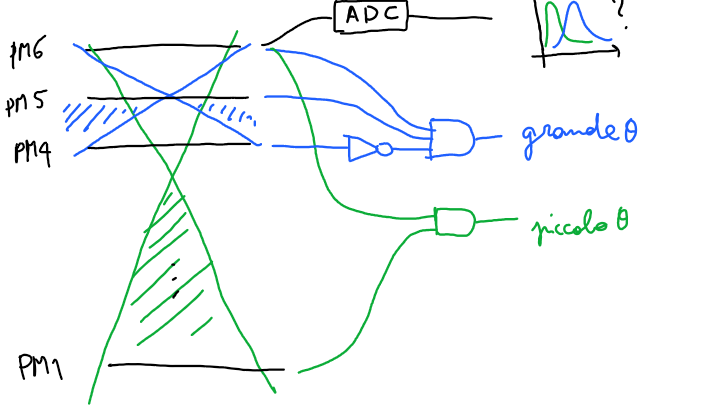
\includegraphics[width=8 cm]{ang}
\caption{Schema della strategia di coincidenze per selezionare l'angolo delle particelle incidenti.}
\label{ang}
\end{figure}

Questo è ciò che abbiamo effettivamente verificato.
Infatti la moda per la distribuzione a grande angolo è $\SI{307\pm7}{mV}$,
mentre quella per angoli piccoli vale $\SI{250\pm5}{mV}$.
La moda è calcolata prendendo il massimo dei bin dell'istogramma e assegnando come incertezza la semilarghezza del bin.
In \autoref{isto} sono presenti gli istogrammi ottenuti dalle due configurazioni di misura.
\begin{figure}
\centering
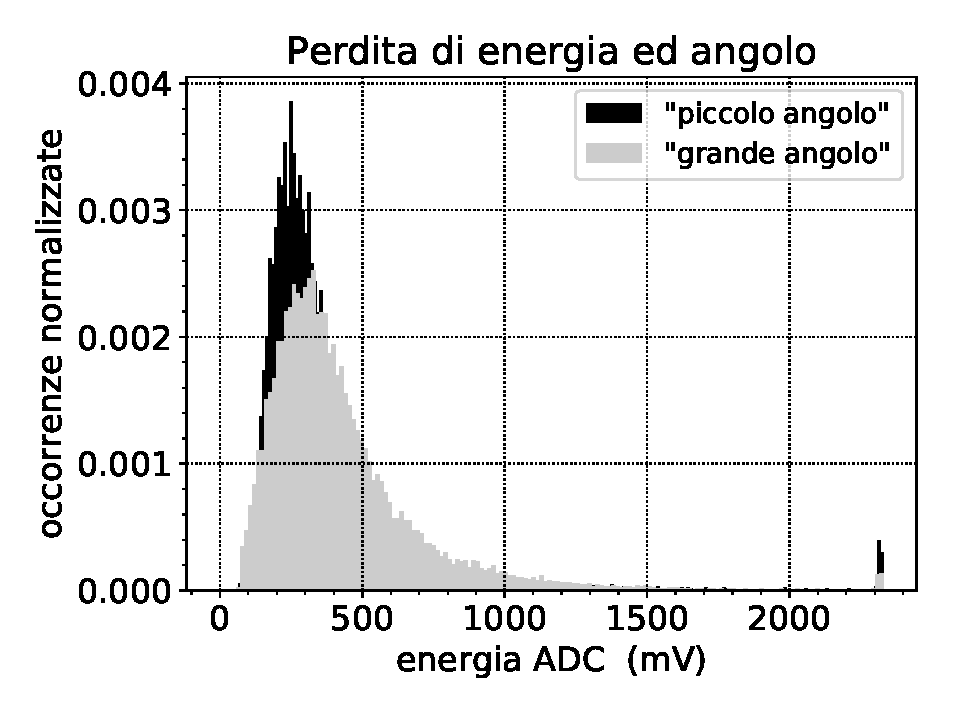
\includegraphics[width=8 cm]{angoli}
\caption{Energia rilasciata per due selezioni angolari dei raggi significativamente diverse.
Il picco presente sulla coda è causato dagli eventi abbastanza energetici da saturare l'uscita dell'amplificatore.
MODIFICA: scala di grigi, ingrandire un pelo, virgolette per piccolo-grande angolo.}
\label{isto}
\end{figure}
